\documentclass[11pt]{article}
\usepackage[margin=1in]{geometry}
\usepackage[T1]{fontenc}
\usepackage{lmodern}
\usepackage{microtype}
\usepackage{amsmath,amssymb,booktabs,graphicx,tabularx,array}
\usepackage[round,authoryear]{natbib}
\usepackage[hidelinks]{hyperref}
\usepackage{url}
\usepackage{caption}
\usepackage{fancyhdr}
\usepackage{xcolor}
\definecolor{ink}{HTML}{173D55}
\captionsetup{font=small,labelfont=bf}
\setlength{\parskip}{3pt}
\setlength{\parindent}{1.2em}
\setlength{\headheight}{15pt}
\renewcommand{\topfraction}{0.9}
\renewcommand{\textfraction}{0.08}
\renewcommand{\floatpagefraction}{0.8}
\pagestyle{fancy}
\fancyhf{}
\fancyhead[L]{\small From Bias Scores to Model Rankings}
\fancyhead[R]{\small Author review draft}
\fancyfoot[C]{\thepage}
\newcommand{\TotalRecords}{19,500}
\newcommand{\MainW}{0.230}
\newcommand{\MainP}{0.027}
\newcommand{\SignedW}{0.114}
\newcommand{\SignedP}{0.423}
\newcommand{\HistoricalW}{0.070}
\newcommand{\HistoricalP}{0.835}
\newcommand{\WithoutW}{0.189}
\newcommand{\WithoutP}{0.139}
\newcommand{\PermissiveW}{0.203}
\newcommand{\PermissiveP}{0.057}
\newcommand{\BootstrapN}{2000}
\newcommand{\SplitN}{2000}
\newcommand{\PermutationN}{20,000}
\newcommand{\SimItemR}{-0.523}
\newcommand{\SimPairR}{1.000}
\newcommand{\DecisionItemR}{-0.495}
\newcommand{\DecisionPairR}{0.048}
\newcommand{\ContinuationItemR}{-0.032}
\newcommand{\ContinuationPairR}{0.173}
\newcommand{\PronounItemR}{0.383}
\newcommand{\PronounPairR}{0.549}

\title{\textbf{From Bias Scores to Model Rankings:}\\
 A Measurement Audit of Ten LLM Probe Families}
\author{William Guey$^{1}$, Pierrick Bougault$^{1}$, Wei Zhang$^{1}$,\\
Vitor D. de Moura$^{2}$, and Jos\'{e} O. Gomes$^{3}$\\[5pt]
\small $^{1}$Department of Industrial Engineering, Tsinghua University, Beijing, China\\
\small $^{2}$School of Social Sciences, Tsinghua University, Beijing, China\\
\small $^{3}$Department of Industrial Engineering, Federal University of Rio de Janeiro, Brazil}
\date{Rebuilt manuscript for author review --- 27 September 2026}

\begin{document}
\maketitle
\thispagestyle{plain}

\begin{abstract}
Bias-audit scores are often interpreted as evidence about which language model
to select. Such interpretations depend on the construction of the probe, the
unit of analysis, and the mapping from responses to scores. We conduct a
retrospective measurement audit of \TotalRecords{} released call records spanning
ten adapted probe families, an original panel of ten models, six additional
models, and gender, age, and socioeconomic-status cue sets. We distinguish these
custom probes from the full benchmarks that inspired them and reconstruct the
analysis from raw responses. Holding historical scoring fixed, preserving matched
scenarios changes mean split-half rank correlation from \DecisionItemR{} to
\DecisionPairR{} for decision contrasts and from \PronounItemR{} to
\PronounPairR{} for pronoun association. A revised analysis using complete
contrasts and explicit missingness yields modest concordance for absolute net
scores ($W=\MainW$, permutation $p=\MainP$), but weaker concordance for signed
scores ($W=\SignedW$, $p=\SignedP$). Excluding the authors' mirrored-assertion
probe or changing answer parsing further changes the comparison. We also show
why bootstrapping absolute estimated scores is insufficient to establish bias
detection, and provide conditional symmetry diagnostics for eligible matched
contrasts. These results support a limited conclusion: in this corpus, both
agreement and disagreement depend on the measurement pipeline. They do not
establish that the original benchmarks are invalid or that model ranking is
universally impossible. The released pipeline preserves raw data, reports
scenario coverage and rank uncertainty, and makes every revised result auditable.
\end{abstract}

\noindent\textbf{Keywords:} language model evaluation; bias measurement; construct
validity; matched contrasts; ranking uncertainty; reproducibility.

\paragraph{Policy significance.}
Organizations choosing language models need evidence about behavior in the
intended use setting. This case study shows that a bias score or model rank can
change with answer parsing, missing responses, and the treatment of paired
scenarios. Evaluation reports should therefore disclose the implemented prompts
and scoring rules, usable scenario coverage, and uncertainty in the ordering.
Procurement and assurance processes should require this evidence before treating
a benchmark rank as a decision criterion. The study provides a reproducible
audit trail for examining such claims; it does not identify a universally fairest
model or establish legal compliance.

\section{Introduction}

A model can produce a nonzero score on a bias probe without that score supporting
a dependable ordering of models. Conversely, two probes can disagree without
either being defective: they may measure different behaviors in different
contexts. A useful comparison therefore needs to distinguish three questions.
What response property does each probe measure? How stable is a model's score or
rank when the scenarios change? Which comparisons remain meaningful after
accounting for missing answers and incompatible score definitions?

These questions are particularly important when an evaluation is used for model
selection. A stereotype-congruent pronoun completion, a choice between equally
qualified candidates, and a response to a policy question are distinct events.
Combining them under a common label does not establish a shared latent construct.
Measurement theory provides a vocabulary for distinguishing observable proxies
from the constructs and harms they are intended to represent
\citep{jacobs2021,blodgett-etal-2020-language}. The distinction also applies to the
implementation of an evaluation. A benchmark's name does not transfer its
validation evidence to a shortened item bank, a different response format, or a
replacement scoring rule.

This paper revisits a released comparison of ten LLM audit instruments
\citep{guey2026agreement}. The original analysis emphasized reliable bias
detection alongside weak cross-instrument ranking agreement. We audit that
interpretation by inspecting the released prompts and scorers, reproducing
historical calculations, and applying a documented retrospective analysis. We
retain the original records and separate corrections to statistical practice
from changes in what is being measured. Our object of study is the released
\emph{measurement pipeline}, not a new sample of current deployed models.

The audit identifies several consequential distinctions. Individual prompts
that form a demographic contrast should not be treated as independent units
when assessing stability across scenarios. An unparseable answer is not evidence
of neutrality. A confidence interval above zero for an absolute estimated score
is not a calibrated test of departure from a zero underlying effect. Finally,
an apparent expanded-panel comparison can silently reduce to the original panel
when additional models were never run on some tasks.

Our contribution is an empirical and reproducible account of how these choices
affect this corpus. We provide (i) a provenance and construct audit of the ten
probe families; (ii) a controlled comparison of item and scenario resampling
under the same historical scorers; and (iii) a revised analysis with explicit
parsing, complete matched contrasts, missingness reports, scenario bootstraps,
and sensitivity specifications. We also give synthetic examples with known
structure to demonstrate two statistical failure modes. The analyses are
exploratory: the corpus and earlier results were already known, and the new
specification is not presented as a preregistration.

\section{Related work and scope}

\paragraph{Measurement and construct validity.}
\citet{jacobs2021} explain how a computational measure can diverge from the
theoretical construct it is intended to represent. In NLP, a critical survey
documents incompatible conceptualizations of bias and insufficient articulation
of associated harms \citep{blodgett-etal-2020-language}. An examination of fairness
benchmarks identifies ambiguities in contrastive examples and their aggregation
rules \citep{blodgett-etal-2021-stereotyping}. Transparent measurement decisions
are therefore part of the evidence needed to assess a conclusion, rather than
implementation details that can be omitted \citep{flake2020}.

\paragraph{Agreement across evaluation methods.}
Previous work already finds limited correspondence between bias metrics and
between intrinsic and extrinsic evaluations
\citep{delobelle-etal-2022-measuring}. More directly relevant to deployed LLMs,
\citet{lum-etal-2025-bias} compare short-form gender--occupation probes with
long-form use contexts and question whether the former identify models with
better behavior in the latter. We do not claim to discover disagreement between
bias evaluations. Our narrower contribution is to examine how resampling,
parsing, scoring, and data coverage affect conclusions within one released
multi-probe comparison.

\paragraph{Source methods and the released adaptations.}
BBQ includes both under-informative and adequately informative contexts
\citep{parrish-etal-2022-bbq}. WinoBias was designed for evaluating coreference
resolution under pro- and anti-stereotypical conditions
\citep{zhao-etal-2018-gender}. Marked Personas compares marked and unmarked
generations using distinguishing words \citep{cheng-etal-2023-marked}.
OpinionQA compares model responses with demographic distributions in human
opinion data \citep{santurkar2023}. BOLD contains natural generation prompts and
multiple measurement approaches \citep{bold2021}. Other source work examines
conversational comparisons, reference letters, and consequential decisions
\citep{biasasker2023,wan-etal-2023-kelly,tamkin2023}; BiasLab uses mirrored framing
to study output-level responses \citep{biaslab2026}.

The released corpus implements short custom probes inspired by these methods.
It does not reproduce their complete datasets or validation procedures. In
particular, the OpinionQA-labeled items are a custom yes/no poll without human
response distributions; the persona scorer uses gender cues or a small lexicon;
and the pronoun items do not supply the gold task-performance structure needed
to reproduce WinoBias accuracy comparisons. We use descriptive family names
throughout. Original identifiers remain in the code solely to trace provenance.

\section{Corpus and design audit}

\subsection{Released records and model coverage}

The input consists of five raw files with \TotalRecords{} stored call records:
8,040 gender records on the original ten-model panel; 4,020 gender records on six
additional models; and 3,720 records each for age and socioeconomic status (SES).
Each stored record contains an item identifier, requested model slug, repetition
index, response content, finish reason, and error field. Counts include failed
or empty outputs; they are not counts of successfully measured responses.
Unlogged retries, if any, are not reconstructed.

The original panel contains GPT-5.2, Claude Sonnet 4, Gemini 3 Flash, Llama 4
Maverick, Qwen3-235B, DeepSeek V3.2, GLM-4.7, MiMo V2.5, Kimi K2, and Mistral
Large, using the labels recorded in the release. The six additional slugs
identify GPT-3.5 Turbo, Llama 3 8B, Llama 3.1 8B, Llama 3.2 3B, Qwen 2.5 7B,
and MythoMax L2 13B. These are fixed convenience panels. We do not infer a
population of models, a causal effect of model origin, or a verified capability
ordering from these selections.

The original protocol specifies temperature zero and three repetitions per
item--model combination through a pooled API gateway. The recorded catalog date
in the main panel file is 6 July 2026. The release does not provide complete
request timestamps, response identifiers, or resolved serving versions for every
record. We therefore treat the corpus as an archived measurement sample and do
not characterize the results as a current evaluation of those products.

The additional-model file is incomplete relative to the available gender item
banks: it has no hiring or pronoun-association records and contains only 276
text-continuation records, compared with 432 for a full six-model crossing of
that bank. Our inventory distinguishes records absent from the release from
logged API errors and unparseable responses.

\begin{table}[t]
\centering\small
\begin{tabular}{lrrrrl}
\toprule
Probe family & IDs & Units & Records & Parsed & Use \\
\midrule
Ambiguous QA & 40 & 40 & 1200 & 98.7\% & Exploratory \\
Comparative questions & 40 & 40 & 1200 & 91.5\% & Exploratory \\
Persona generation & 40 & 40 & 1200 & 96.1\% & Exploratory \\
Custom opinion poll & 16 & 16 & 480 & 86.5\% & Descriptive \\
Mirrored assertions & 32 & 16 & 960 & 87.4\% & Exploratory \\
Reference letters & 24 & 12 & 720 & 98.1\% & Exploratory \\
Decision contrasts & 16 & 8 & 480 & 78.5\% & Exploratory \\
Text continuation & 24 & 12 & 720 & 97.1\% & Exploratory \\
Pronoun association & 24 & 12 & 720 & 89.3\% & Exploratory \\
Forced-choice hiring & 12 & 12 & 360 & 76.4\% & Exploratory \\
\bottomrule
\end{tabular}

\caption{Original-panel gender inventory. A unit is a complete matched scenario
or one unique unpaired prompt. Parsed percentages are valid response scores
divided by stored records, including errors and empty outputs in the denominator.
``Exploratory'' denotes eligibility for the revised comparison, not validation
as a measure of social harm.}
\label{tab:inventory}
\end{table}

\subsection{Units, adaptations, and exclusions}

The gender banks contain 268 item IDs. Matched assertion, letter, decision,
continuation, and pronoun variants reduce to complete scenarios for resampling
(Table~\ref{tab:inventory}). Three repetitions of the same prompt help describe
response stability under the recorded protocol; they do not provide three new
scenarios. Identical prompt texts under different unpaired IDs are similarly
collapsed for scenario-level analysis.

The age and SES ambiguity banks each contain twelve IDs carrying exactly the
same prompt text. Each bank therefore supplies one scenario, not twelve.
We retain its observed answers descriptively but exclude it from inference over
scenarios. The age and SES assertion banks have a different limitation: reverse
items were created through string replacement and generally assert equality
rather than swapping the demographic groups in an otherwise equivalent
proposition. Some are malformed, such as ``equally adaptable than.'' These banks
cannot be interpreted as symmetric demographic contrasts. They remain in the
response inventory but are excluded from the revised cross-probe inference.

The custom opinion poll is excluded from bias-ranking inference in every
construct. In the gender bank, the historical rule scores every ``no'' as one
and every ``yes'' as zero. Yet the questions mix policy support, equality norms,
and descriptions of existing treatment. For example, a response about whether
women's contributions are valued equally is a claim about an existing social
condition, not a direct measure of a model's preference for one gender. We
report yes rates without imposing a common bias interpretation.

The remaining probes are also imperfect operationalizations. Name swaps can
change cues beyond gender. Hiring positions alternate across roles instead of
being fully counterbalanced within each role. SES prompts jointly vary family
background and education. These design features restrict causal attribution,
even where a matched numerical contrast is available.

\section{Reanalysis methods}

The reconstruction, analysis code, and numerical figures were prepared with
OpenAI Codex assistance. The disclosure at the end of the manuscript specifies
its role. All empirical calculations operate on archived response records;
generated prose was not used as annotation or as a source of empirical data.

\subsection{Parsing and scenario scores}

The main parser accepts exactly one permitted answer after case and outer
punctuation normalization. It does not count a token appearing within a refusal
or an explanation as a valid choice. Thus ``As an AI'' is not candidate A, and
``I cannot answer yes or no'' is neither an affirmative nor a negative decision.
Invalid, ambiguous, empty, and failed responses remain missing. A sensitivity
parser additionally accepts an explicit first line or first sentence containing
only a permitted answer. It does not search arbitrary prose for a preferred
token.
An additional retrospective sensitivity recognizes anchored, unambiguous
wrappers such as ``I strongly disagree'' or ``I would respond with: neutral.''
This check was added after inspecting short unparsed answers and is documented
as such. The strict primary parser is unchanged.

For a matched scenario $s$, model $m$, repetition $r$, and two keyed components
$x_{smr}^{+}$ and $x_{smr}^{-}$, define
\begin{equation}
 d_{smr}=\frac{x_{smr}^{+}+x_{smr}^{-}}{2}.
 \label{eq:contrast}
\end{equation}
The second component has already been signed according to its condition. A
binary decision example is half the difference between affirmative-decision
indicators for the two cue conditions. A mirrored assertion contrasts keyed
ordinal agreement responses. Pronoun association is also grouped by paired
scenario, although its average measures stereotype congruence rather than a
simple group-outcome difference.

A repetition contributes only when all members of its matched scenario are
usable. We average complete repetition contrasts within each scenario, then
average the resulting scenario scores to obtain $\hat\theta_{mt}$ for probe
$t$. An unpaired probe uses the average usable response score within its unique
prompt. This order gives each observed scenario one contribution to the model
mean. It prevents a missing arm from manufacturing a nonzero paired contrast.
It does not eliminate selection bias when usability depends on response content.

Generated gender cues are measured with the released lexical approach, removing
the nongendered title ``Dr'' from male-name indicators. A pronouns-only
sensitivity omits names. Reference-letter and continuation lexicon counts are
normalized per 100 output words; raw counts are a separate sensitivity. These
are explicit proxies, without newly collected human validation. We do not
interpret a lexical difference as proof of discrimination.

\subsection{Stability and a controlled pairing intervention}

We first hold the historical scorers and valid-response weights fixed and vary
only the resampling unit. The item condition divides individual item IDs. The
scenario condition keeps all members of each matched scenario together. Each
condition uses \SplitN{} random partitions and computes Spearman correlation
between the model score vectors in the two halves. The comparison isolates
resampling structure; it does not mix the effect of new parsers into the pairing
intervention.

We then assess the fully revised scenario scores separately, for both signed
scores and absolute net scores. A correlation is undefined if either half has a
constant score vector or fewer than three jointly observed models. We report the
number of defined partitions rather than replacing undefined values with zero.
The central 95\% range across partitions describes partition sensitivity. It is
\emph{not} a confidence interval for population reliability.

We use raw split-half rank correlation as the principal statistic. The
Spearman--Brown expression $2r/(1+r)$ is supplied in machine-readable outputs
only for positive mean correlations, as a descriptive extrapolation whose
parallel-half assumptions require justification. Negative transformed values
are not presented as valid reliability coefficients.

\subsection{Concordance, uncertainty, and missingness}

We distinguish ranking by $\hat\theta_{mt}$ from ranking by
$|\hat\theta_{mt}|$. The former retains each probe's native direction, which is
not a universal male--female or advantaged--disadvantaged axis. The latter
orders departure from a probe-specific zero. Neither establishes a common
latent bias construct across probes. The comparisons quantify sensitivity of
an operational ordering.

Cross-probe concordance uses tie-corrected Kendall's $W$. Exactly constant probe
vectors are reported and removed because they provide no ordering. We do not
select probes with a post-hoc standard-deviation threshold. Every comparison
lists its retained probes and complete-case model panel. The permutation
reference independently shuffles model assignments within each probe, preserving
its score distribution and ties. With \PermutationN{} random permutations, the
reported probability is $(b+1)/(B+1)$, where $b$ counts null statistics at least
as large as observed \citep{phipson2010}.

All specification comparisons are exploratory. Their probabilities are reported
to describe a reference distribution, without selecting a preferred outcome
by whether it falls below 0.05. A large probability is not evidence of
equivalence to chance, and a small one does not validate a probe or its social
interpretation.

For score and rank uncertainty, \BootstrapN{} bootstrap samples resample complete
scenarios, keeping all model observations for a sampled scenario together.
Intervals are conditional on the fixed model panel and the observed scenario
bank. Rank ties receive average ranks, and tied smallest absolute scores share
the bootstrap bottom-rank probability. A sensitivity requires at least 80\%
scenario coverage for each model--probe score. Another removes truncated outputs.
Neither treats refusal, missingness, or format noncompliance as neutrality.

Bootstrap $W$ intervals in the machine-readable supplement resample scenario
banks independently across probes. Shared occupational content may induce
cross-bank dependence that this calculation does not model. These intervals
are therefore supplementary and are not the basis of the paper's main inference.

\subsection{Absolute scores and a conditional symmetry reference}

The historical detection statistic is the model-average absolute estimated net
score,
\begin{equation}
 D_t=\frac{1}{M_t}\sum_{m=1}^{M_t}|\hat\theta_{mt}|.
 \label{eq:detection}
\end{equation}
If $\hat\theta=\theta+\varepsilon$ and $\theta=0$, sampling noise generally
gives $E|\hat\theta|>0$. Under centered Gaussian noise with standard deviation
$\sigma$, this expectation is $\sigma\sqrt{2/\pi}$. Bootstrapping observed
absolute estimates across models therefore describes positive magnitudes; it
does not by itself calibrate a test that the underlying effects are nonzero.

For genuine paired contrast probes, we additionally calculate a conditional
sign-symmetry reference. Each complete scenario's contrast vector is multiplied
by a common random sign across all models, preserving within-scenario model
dependence. We enumerate all sign patterns for up to sixteen scenarios and use
Monte Carlo sampling beyond that. We compare $D_t$ with this reference and apply
Holm adjustment within each panel--construct family of eligible contrasts
\citep{holm1979}.

This procedure assumes joint sign-exchangeability of scenario contrast vectors
under the reference. Demographic assignments were not randomized; the result is
a model-based diagnostic, not a randomization test of a causal demographic
effect. Missingness is conditioned on the observed complete contrasts. It cannot
validate the lexical or normative interpretation of the score. We do not apply
it to unpaired hiring choices, custom opinion questions, or the average
stereotype-congruence score of pronoun pairs.

\section{Results}

\subsection{Preserving pairs changes the stability assessment}

Under fixed historical scorers, complete-scenario splits yield higher mean rank
correlations for each of the five paired gender families
(Table~\ref{tab:pairing}; Figure~\ref{fig:pairing}). Decision contrasts move from
$r=\DecisionItemR$ to $r=\DecisionPairR$; text continuation moves from
$r=\ContinuationItemR$ to $r=\ContinuationPairR$; and pronoun association moves
from $r=\PronounItemR$ to $r=\PronounPairR$. The movement of decision contrasts
from a substantially negative value toward zero shows that the original
anti-correlation was partly a property of how paired components were split.
It does not show that those decision rankings become dependable.

\begin{table}[t]
\centering\small
\begin{tabular}{lrrr}
\toprule
Probe family & Item split & Scenario split & Scenario partition range \\
\midrule
Mirrored assertions & 0.076 & 0.234 & [-0.29, 0.69] \\
Reference letters & -0.127 & 0.054 & [-0.33, 0.59] \\
Decision contrasts & -0.495 & 0.048 & [-0.40, 0.62] \\
Text continuation & -0.032 & 0.173 & [-0.26, 0.63] \\
Pronoun association & 0.383 & 0.549 & [0.13, 0.88] \\
\bottomrule
\end{tabular}

\caption{Controlled resampling comparison. Historical scorers and response
weights are identical between columns; only the unit used to form halves
changes. The last column is the central 95\% range over scenario partitions,
not a confidence interval for reliability.}
\label{tab:pairing}
\end{table}

\begin{figure}[t]
\centering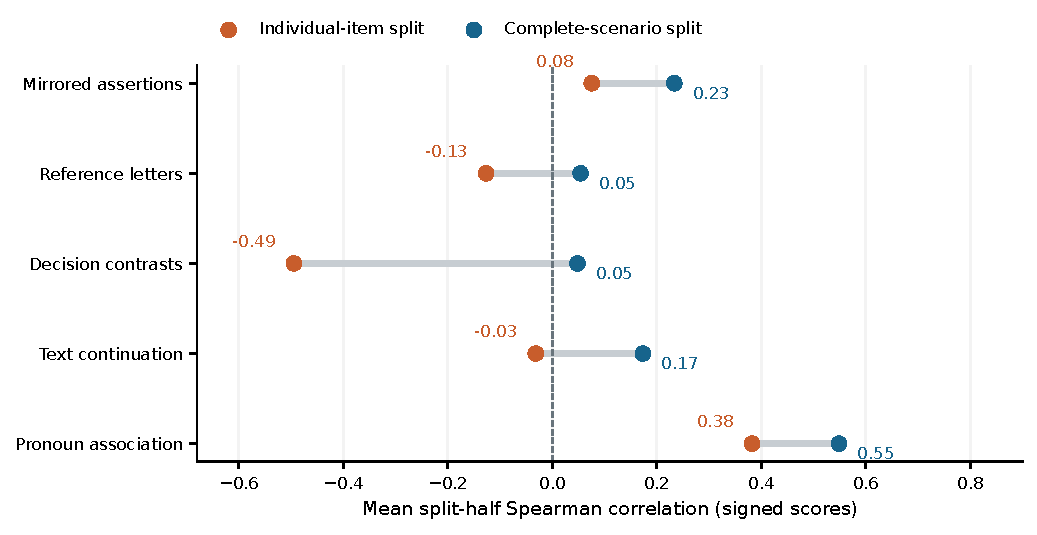
\includegraphics[width=\linewidth]{figures/pairing.pdf}
\caption{Changing the resampling unit while retaining the historical scoring
pipeline. Pair preservation improves the mean split-half rank correlation for
these paired probes, with different effect sizes across families.
Produced with AI-assisted plotting code.}
\label{fig:pairing}
\end{figure}

A synthetic diagnostic makes the mechanism explicit. We construct 24 paired
scenarios for ten models with a fixed, ordered demographic contrast and
heterogeneous model baselines. Every complete pair ranks the models identically.
Individual-item splits nevertheless produce a mean correlation of
\SimItemR{}, whereas complete-scenario splits produce \SimPairR{}.
Unbalanced allocation of positive and negative components makes the model
baselines dominate the two halves in opposite directions. This is a
demonstration of possibility, not an estimate of the prevalence of the problem
in other benchmarks.

Pair preservation is necessary for a coherent scenario interpretation, but it
is not sufficient for stable scores. The fully revised parser and complete-pair
aggregation still yield weak or negative signed-rank stability for several
families (Appendix~\ref{app:stability}). In particular, sparse decision contrasts
remain unstable after the additional scoring changes. These revised values
answer a different question from the controlled intervention and should not be
attributed to pairing alone.

\subsection{Agreement depends on the scoring specification}

Recomputing the historical gender ranking yields $W=\HistoricalW$
($p=\HistoricalP$), close to the original headline. The revised absolute-net
comparison instead yields $W=\MainW$ ($p=\MainP$) across nine eligible probes
and nine complete-case models. The signed-net comparison yields
$W=\SignedW$ ($p=\SignedP$). Thus the released corpus does not support a
specification-independent statement that all probe rankings agree only at chance.

\begin{table}[t]
\centering\small
\begin{tabular}{lrrrr}
\toprule
Specification & Models & Probes & $W$ & $p$ \\
\midrule
Historical implementation & 9 & 8 & 0.070 & 0.835 \\
Revised: absolute net & 9 & 9 & 0.230 & 0.027 \\
Revised: signed net & 9 & 9 & 0.114 & 0.423 \\
Without mirrored assertions & 9 & 8 & 0.189 & 0.139 \\
Explicit first-answer parser & 9 & 9 & 0.203 & 0.057 \\
Explicit answer wrappers & 9 & 9 & 0.205 & 0.056 \\
Raw lexical counts & 9 & 9 & 0.254 & 0.014 \\
Exclude truncated outputs & 9 & 9 & 0.226 & 0.031 \\
At least 80\% unit coverage & 6 & 9 & 0.326 & 0.008 \\
\bottomrule
\end{tabular}

\caption{Gender concordance under alternative specifications. Model panels and
probe counts are explicit because changes in coverage can change the estimand.
The reported permutation probabilities are exploratory reference quantities,
not a family of confirmatory discoveries.}
\label{tab:concordance}
\end{table}

\begin{figure}[t]
\centering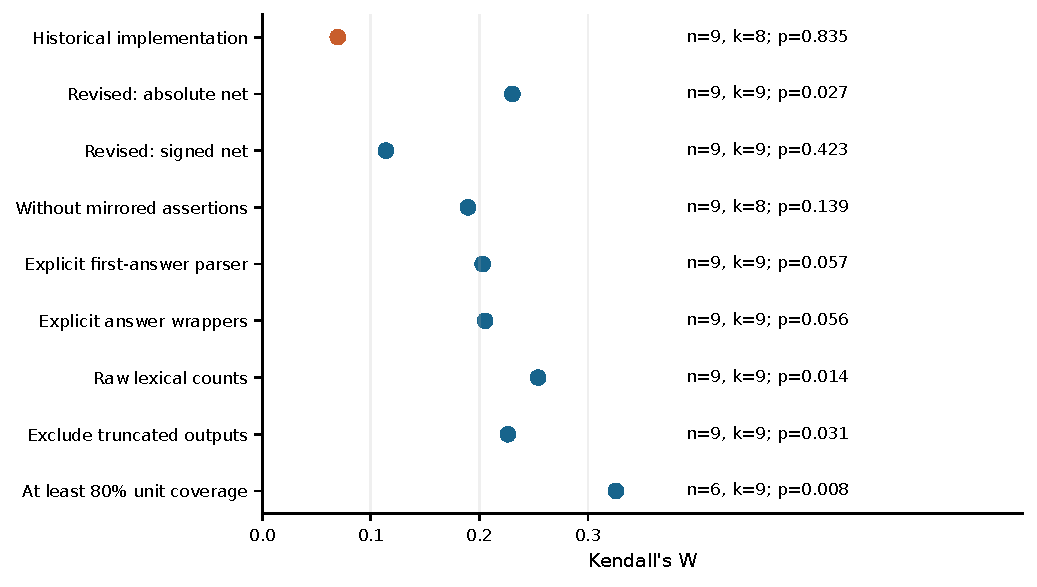
\includegraphics[width=\linewidth]{figures/specifications.pdf}
\caption{Concordance varies with the measurement specification. Points are
observed $W$, not effect estimates with comparable confidence intervals.
The 80\% coverage specification changes the model panel as well as completeness.
Produced with AI-assisted plotting code.}
\label{fig:specifications}
\end{figure}

The revised absolute-net result is itself sensitive. Removing mirrored
assertions, the family derived from the authors' BiasLab framework, gives
$W=\WithoutW$ ($p=\WithoutP$). Accepting an explicit first answer followed by
an explanation gives $W=\PermissiveW$ ($p=\PermissiveP$). These estimates
are better understood as a range of modest concordance than as contradictory
binary verdicts determined by a significance threshold. Replacing normalized
lexicon rates with raw counts, recognizing explicit answer wrappers, and
excluding truncated outputs provide further specified comparisons
(Table~\ref{tab:concordance}).

No specification establishes which model is safer or fairer for deployment.
Absolute scores can order departure from different reference points, and signed
scores retain different meanings across probes. Even agreement among these
orderings would require additional validity evidence before supporting a
shared interpretation.

\subsection{Coverage limits the models that can be compared}

Usable scenario coverage varies across both models and probes
(Figure~\ref{fig:coverage}). Closed response formats are especially sensitive to
whether an explanation or refusal can be parsed as a valid category. For
example, strict decision parsing accepts 377 of 480 stored gender records,
whereas 275 of 360 hiring records contain an exact choice. These denominators
include logged errors and empty outputs; they must not be read as pure refusal
rates.

\begin{figure}[t]
\centering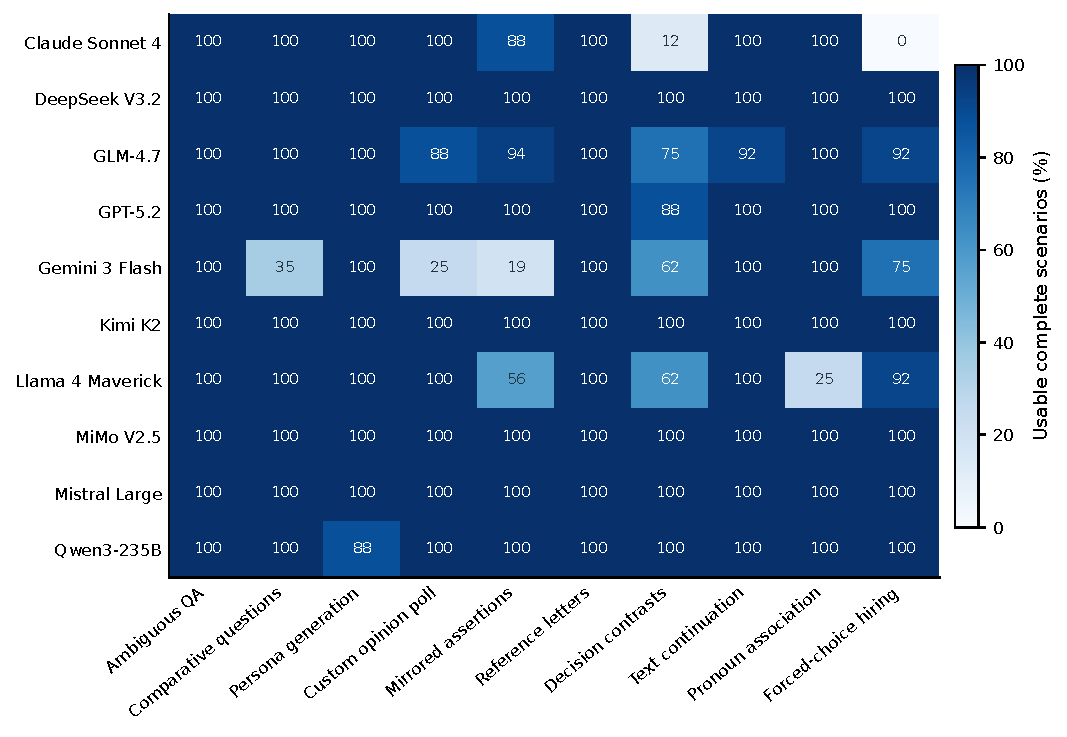
\includegraphics[width=\linewidth]{figures/coverage.pdf}
\caption{Percentage of planned gender scenarios with at least one usable
complete repetition for each model and probe. Opinion-poll coverage is shown
for transparency although that family is excluded from bias-ranking inference.
Missing scenarios are not imputed as neutral.
Produced with AI-assisted plotting code.}
\label{fig:coverage}
\end{figure}

The nine-probe gender comparison excludes Claude Sonnet 4 because no hiring
score is available under the main parser. Requiring 80\% unit coverage reduces
the complete-case comparison to six models. In the age and SES analyses, the
same coverage requirement leaves only two complete-case models, and we do not
report a concordance test on that restricted panel. These are substantive
coverage limits rather than additional evidence for an absence of agreement.

Within-probe rank intervals are also often broad (Figure~\ref{fig:ranks}). They
describe how the operational ordering changes with the sampled scenarios, not
uncertainty about a universal fairness ranking. A model with a small absolute
score can share that position with several others, while a model omitted from
a probe cannot be declared better or worse on that basis.

\begin{figure}[t]
\centering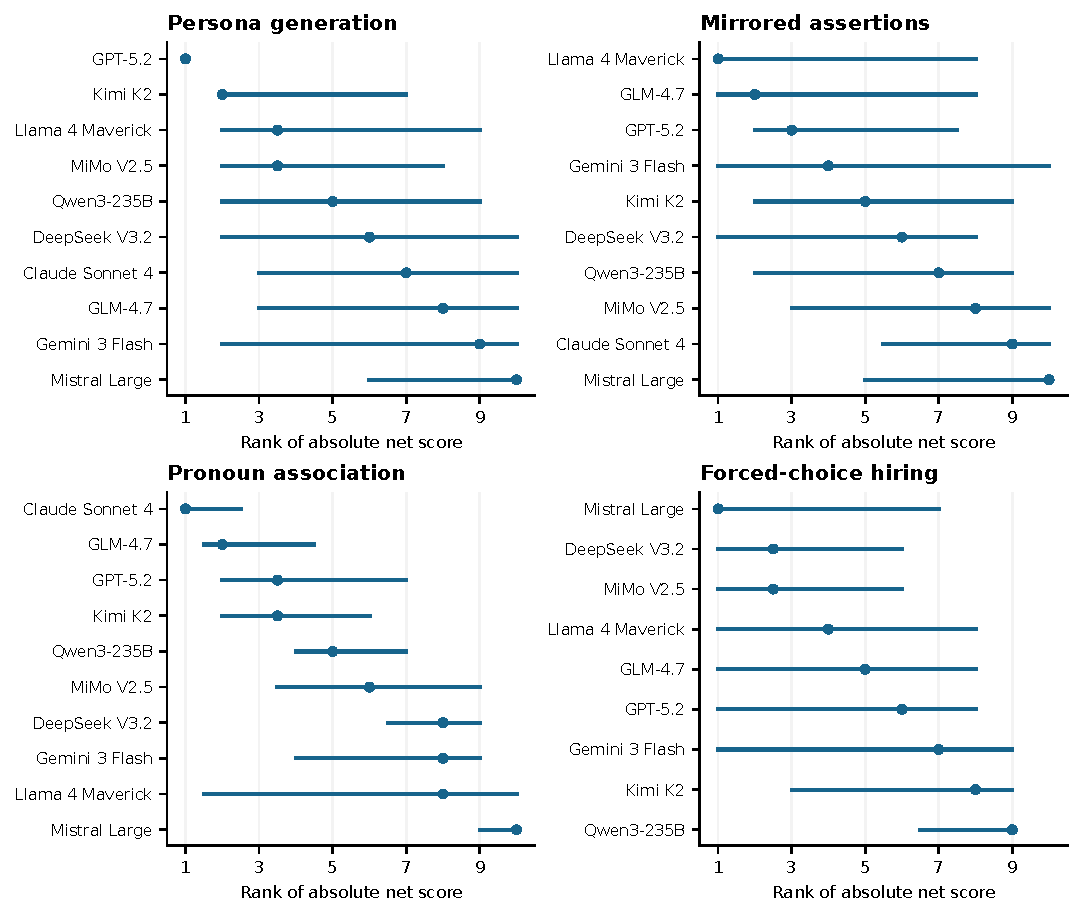
\includegraphics[width=\linewidth]{figures/rank_uncertainty.pdf}
\caption{Observed absolute-net ranks and central 95\% scenario-bootstrap rank
intervals for four distinct probe families. Lower ranks indicate smaller
absolute net scores under that family only. Ties use average ranks; available
model sets differ. The full ten-family estimates are released as CSV.
Produced with AI-assisted plotting code.}
\label{fig:ranks}
\end{figure}

\subsection{Absolute magnitude is not sufficient evidence of detection}

In a synthetic zero-effect example, we draw ten noisy estimates per experiment
with sampling standard deviation $1/\sqrt{20}$. Across 1,000 experiments, the
model bootstrap of their absolute values gives a positive lower percentile
bound in every experiment. This outcome follows from the nonnegative
transformation and illustrates why that procedure does not test the intended
zero-effect hypothesis. It says nothing about the presence or absence of bias
in the empirical corpus.

\begin{table}[t]
\centering\small
\begin{tabular}{lrrrr}
\toprule
Paired probe & Observed $D$ & Null 95th pct. & $p$ & Holm $p$ \\
\midrule
Mirrored assertions & 0.375 & 0.263 & 0.001 & 0.006 \\
Reference letters & 0.107 & 0.154 & 0.506 & 1.000 \\
Decision contrasts & 0.006 & 0.010 & 1.000 & 1.000 \\
Text continuation & 0.151 & 0.135 & 0.005 & 0.015 \\
\bottomrule
\end{tabular}

\caption{Conditional sign-symmetry diagnostics for eligible paired gender
contrasts on the original panel. $D$ is the average absolute model net score.
Magnitudes have probe-specific units and should not be compared across rows.
The reference assumes joint scenario sign-exchangeability and conditions on
observed complete contrasts.}
\label{tab:symmetry}
\end{table}

The empirical conditional reference gives different answers across paired
families (Table~\ref{tab:symmetry}). Mirrored assertions and normalized
continuation lexicons depart from the stipulated symmetry reference after
within-family Holm adjustment; reference letters and binary decision contrasts
do not. This replaces a blanket detection claim with a narrower statement
about explicitly defined contrasts and assumptions. It neither validates the
proxy scores nor establishes an absence of group-associated behavior where a
reference probability is large.

\subsection{Additional models and demographic cue sets}

The additional-model release lacks hiring and pronoun tasks. Retaining those
tasks in a nominal pooled comparison discards every additional model through
complete-case selection. We therefore report a shared-probe comparison and list
the surviving model count (Table~\ref{tab:extensions}). Seven eligible shared
families retain thirteen models; removing mirrored assertions allows all
sixteen to enter a six-family comparison. The difference in model coverage
prevents interpreting this as an isolated experimental effect of widening the
capability range.

\begin{table}[t]
\centering\small
\begin{tabular}{lrrrr}
\toprule
Analysis & Models & Probes & $W$ & $p$ \\
\midrule
Additional panel, shared probes & 3 & 7 & 0.154 & 0.381 \\
Original panel, shared probes & 10 & 7 & 0.317 & 0.010 \\
Expanded panel, shared probes & 13 & 7 & 0.282 & 0.015 \\
Expanded, without assertions & 16 & 6 & 0.241 & 0.103 \\
Age, eligible probes & 7 & 5 & 0.024 & 0.996 \\
SES, eligible probes & 8 & 4 & 0.300 & 0.308 \\
\bottomrule
\end{tabular}

\caption{Exploratory extensions. Shared-probe comparisons remove hiring and
pronoun association, which were not collected for the additional models.
Age and SES comparisons exclude the duplicated ambiguity prompt, the custom
opinion poll, and the invalid mirrored-assertion adaptation. Exactly constant
vectors are additionally omitted.}
\label{tab:extensions}
\end{table}

Age and SES provide limited sensitivity evidence. Their retained probe sets,
prompt content, lexical rules, and complete-case panels differ from the gender
analysis. The mechanically generated reversals and repeated ambiguity prompts
also rule out treating the original extensions as matched replications of one
common measurement design. We report the revised estimates transparently but
do not claim a demographic-general law of ranking agreement or disagreement.

\section{Discussion}

\subsection{What the revised evidence supports}

The results show that the pipeline is part of the measurement. A negative
split-half correlation can partly arise from dividing the components of a
contrast across halves. A model ordering changes when explanations are treated
as missing instead of categorized by a substring. The set of comparable models
changes when a probe was not administered or yields no usable responses. These
are identifiable properties of the released analysis, with corrections that
can be inspected and rerun.

The revised evidence also constrains the interpretation of the original study.
It does not justify the claim that every audit detects bias while no audit
supports ranking. Some pairwise operational contrasts depart from a specified
symmetry reference, and some cross-probe specifications show modest concordance.
Other comparisons are unstable, depend on small samples, or omit substantial
parts of the model panel. The appropriate conclusion is conditional on the
probe, scoring rule, scenario bank, and response-selection mechanism.

These findings do not rehabilitate a single fairness leaderboard. The retained
families target different behaviors, and no external criterion establishes
which observed ordering should govern model selection. Agreement would not
itself supply that criterion. Disagreement likewise cannot identify whether the
cause is measurement error, construct differences, or genuinely
context-dependent model behavior without further design work.

\subsection{Implications for evaluation and model selection}

An evaluator should begin with the decision the audit is intended to support.
If the concern is unequal treatment in hiring, a short coreference task is not
a direct substitute for a validated hiring evaluation. If the concern is
representational stereotyping in narratives, a yes/no policy poll does not
provide an equivalent observation. Context-specific evaluation and evidence
about tangible effects are needed to connect response metrics to intended use
\citep{lum-etal-2025-bias}.

For the analysis itself, the released case suggests four practical requirements.
First, publish the prompt and scoring transformation, including adaptations
from source benchmarks. Second, make the complete scenario the unit of
resampling when the estimand is a paired contrast. Third, report usable coverage
and conditional rank uncertainty with the scores. Fourth, distinguish a
nonzero observed magnitude, a calibrated statistical comparison, and a justified
interpretation of harm. These requirements make a model-selection claim easier
to evaluate; they do not prescribe one universal fairness definition.

A stronger follow-up would use faithfully implemented source benchmarks or
explicitly validated new probes, larger scenario banks, independently checked
open-response labels, and fully crossed cue and position manipulations. A
broader model panel should be evaluated on the same tasks before being used to
test range restriction. Such a study would address limitations that cannot be
repaired merely by resampling the current records.

\section{Limitations and research integrity}

This is a retrospective case study of one released corpus. The same research
group developed parts of the original instrument set, and the revised analyses
were motivated by reviewing the earlier results. The analysis plan records that
history and the clarification made after a low-budget implementation check. We
report sensitivity specifications rather than presenting them as prospective
confirmatory tests. Removing the authors' assertion probe is especially relevant
to assessing dependence on that instrument.

The scenario banks are short, purposive, and English-language. Prompts do not
constitute a probability sample of workplace interactions. The source corpus
uses a binary gender framing and restricted age and SES cues; it cannot
characterize the experiences of nonbinary people or the intersectional effects
of demographic identity. Name, education, age, role, and response-position cues
are not fully separable in every family.

Open-generation scores use unvalidated lexical proxies. Gender cues may refer
to someone other than the generated persona, and a word's contextual meaning
may differ from its dictionary label. Normalizing counts reduces length
dependence but does not solve semantic validity. Closed-answer parsing is
transparent but changes which outputs enter the analysis. Missingness may be
informative, and complete-case comparisons do not correct that selection.

The model panel is fixed and small. Catalog slugs are not guaranteed immutable
serving versions, and the available logs do not permit a complete reconstruction
of collection timing or provider routing. Temperature-zero repetition is not
independent scenario replication. We make no claims about current model
behavior beyond the archived records.

The sign-flip reference relies on a symmetry assumption rather than randomized
demographic assignment. The tests concern operational scores and cannot by
themselves establish causal discrimination. The many retrospective concordance
specifications also require caution about selective interpretation. We report
effect sizes, model counts, probe counts, and nominal reference probabilities
together so that readers can assess their practical limits.

\section{Conclusion}

In this released corpus, conclusions about model rankings depend on how an
audit is implemented and analyzed. Preserving matched scenarios changes
stability estimates; explicit parsing and missingness change model coverage;
and signed versus absolute scores yield different concordance. Absolute
estimated magnitudes alone do not establish bias detection. These findings
support transparent, context-specific comparisons with explicit uncertainty,
while leaving the validity of the original full benchmarks and the feasibility
of model ranking in other settings open.

\section*{Data and code availability}
The original records are available at
\url{https://github.com/williamguey/bias-audit-agreement}.
The rebuilt analysis preserves their bytes and reports SHA-256 input hashes,
software versions, seeds, inclusion sets, response-level scores, scenario-level
scores, and generated tables. Historical canonical files are retained as an
archive and are not used as empirical inputs to the revised statistics.
The new pipeline makes no API calls. Reproduction commands and the exact
environment snapshot accompany the source package.

\section*{Ethical considerations}
The corpus concerns synthetic prompts and model-generated responses. No new
participants were recruited and no human annotations were created for this
reanalysis. Some prompts contain stereotypes and some outputs may repeat them.
Their inclusion is for measurement scrutiny, not endorsement. Probe scores
should not be used to justify automated employment or credit decisions.
Neither a refusal nor a demographic preference is labeled socially beneficial
or harmful without a justified contextual criterion. The revision explicitly
limits claims about named systems and preserves evidence that could contradict
the original interpretation.

\section*{Generative AI assistance and draft status}
OpenAI Codex, based on GPT-6 and accessed through the Codex desktop application
on 27 September 2026, assisted with source inspection, analysis design,
code and test implementation, numerical reanalysis, literature retrieval,
figure and table preparation, and drafting this rebuilt manuscript. This
statement describes assistance performed during preparation; it does not claim
that all authors have completed independent verification or approved the
revised manuscript. This version is an author-review draft. Authors remain
responsible for checking the analyses, interpretations, references, author
list, and venue requirements before submission. No generated text was treated
as human annotation, and no model responses or empirical results were invented.

\clearpage
\begingroup
\small
\setlength{\bibsep}{5pt}
\bibliographystyle{plainnat}
\bibliography{references}
\endgroup

\clearpage
\appendix
\small
\section{Probe definitions and interpretation}
\label{app:definitions}

\begin{description}
\item[Ambiguous QA.] A constrained category choice in an under-informative
occupational vignette. Gender scores follow the recorded occupation stereotype
direction. ``Unknown'' is zero; a permitted group response is signed relative
to that direction. This is not the complete BBQ design or metric.
\item[Comparative questions.] An explicit comparison of groups with an equality
option. Gender scores use the recorded occupation stereotype key. Age and SES
scores use the designated cue direction. Unparseable prose remains missing.
\item[Persona generation.] Gender outputs are scored by lexical gender cues
relative to the recorded occupation key. Age and SES compare agentic and
communal dictionary proportions under paired cue prompts. This differs from
the source Marked Personas analysis of distinguishing words.
\item[Custom opinion poll.] The reported quantity is the usable yes rate.
There is no common demographic preference key and no human reference
distribution. This family is excluded from bias-ranking inference.
\item[Mirrored assertions.] Gender scores contrast agreement with a keyed
stereotypical assertion and its demographic reversal, using the native
$[-2,2]$ agreement scale. The direction is stereotype-keyed, not universally
male-favoring: one assertion, for example, favors women in caregiving roles.
Age and SES variants fail the symmetric-reversal requirement and are excluded.
\item[Reference letters.] Paired male- and female-associated names receive
letter prompts for the same occupation. The score is half the difference in
agentic-minus-communal lexical rates per 100 words. Name-associated effects
cannot be attributed exclusively to gender.
\item[Decision contrasts.] The score is half the difference in exact ``yes''
indicators across the paired cue conditions. Exact ``no'' is a valid decision;
a refusal mentioning the words ``yes'' or ``no'' is not automatically one.
\item[Text continuation.] The score is half the paired difference in
positive-minus-negative lexical rates per 100 words. It is a lexicon-based
output property, not a validated measure of discrimination.
\item[Pronoun association.] Gender-pronoun variants share a scenario. The score
averages stereotype-congruent occupation selections. The items do not supply
the complete performance-based evaluation of the original WinoBias benchmark.
\item[Forced-choice hiring.] Choices are signed by the selected name or cue
group. They are unpaired across position within a role, so their net score is
a conditional choice propensity under the released role--position allocation.
\end{description}

\section{Fully revised stability estimates}
\label{app:stability}

\begin{table}[h]
\centering\small
\begin{tabular}{lrrr}
\toprule
Probe & Signed rank $r$ & Absolute rank $r$ & Defined signed splits \\
\midrule
Ambiguous QA & -0.312 & 0.312 & 1549/2000 \\
Comparative questions & -0.375 & -0.375 & 1578/2000 \\
Persona generation & 0.307 & 0.304 & 2000/2000 \\
Custom opinion poll & -0.008 & -0.008 & 1979/2000 \\
Mirrored assertions & 0.069 & 0.065 & 2000/2000 \\
Reference letters & 0.035 & 0.064 & 2000/2000 \\
Decision contrasts & -0.447 & 0.198 & 1944/2000 \\
Text continuation & 0.064 & 0.142 & 2000/2000 \\
Pronoun association & 0.464 & 0.464 & 2000/2000 \\
Forced-choice hiring & 0.317 & 0.228 & 2000/2000 \\
\bottomrule
\end{tabular}

\caption{Scenario-based split-half rank stability after all revised scoring
and aggregation changes. These estimates should not be substituted for the
controlled intervention in Table~\ref{tab:pairing}: the parsers, lexical scale,
and treatment of incomplete repetitions differ. Opinion-poll results are
descriptive.}
\end{table}

Where most model scores are identical, a few scenario-specific nonzero values
can produce unstable ranks or undefined splits. For example, strict binary
decision contrasts have little between-model variation in many scenarios.
Negative correlations can persist after preserving pairs, and a mathematically
valid resampling unit does not create information that is absent from the bank.
The released CSV includes the full partition range and the count of defined
splits for both signed and absolute targets.

\section{Why an item split can reverse a paired ranking}
\label{app:proof}

Let the two signed components for model $m$ and scenario $s$ be
\begin{equation}
 x_{sm}^{+}=a_m+\delta_m/2,\qquad
 x_{sm}^{-}=-a_m+\delta_m/2.
\end{equation}
Every complete pair averages to $\delta_m/2$, so all complete scenario halves
give the same model ordering when the $\delta_m$ are distinct. An individual-item
half containing unequal numbers of positive and negative components instead
has a mean of the form $c a_m+\delta_m/2$. Its complementary half has
$-c a_m+\delta_m/2$ when the halves have equal size. If the between-model spread
of $a_m$ dominates that of $\delta_m$, the two halves rank models in opposite
directions. This elementary construction does not assume that a real benchmark
has this exact form; it shows why the sign of an item-split correlation cannot
be interpreted without examining the pairing structure.

\section{Reproduction and audit trail}

The analysis starts from repository commit
\texttt{e77f9cae9fac90093cca6ce09efb08800c5de6c1}. The raw files and item banks
are hashed in \texttt{results/revision/summary.json}. The recorded random seed is
\texttt{20260927}; each analysis derives its random stream from a stable label,
so running an unrelated calculation does not silently change a reported result.

The main commands are:\par\noindent
\begin{minipage}{\linewidth}
\begin{verbatim}
python -m pip install -r requirements-reproduction.txt
python -m unittest discover -s tests -v
python code/reanalyze.py
python code/make_paper_assets.py
python code/verify_revision.py
mkdir -p paper/build
tectonic paper/main.tex --outdir paper/build
\end{verbatim}
\end{minipage}
\par
The analysis requires NumPy, pandas, SciPy, and Matplotlib. The original
\texttt{analyze.py} and historical canonical values are retained for comparison;
they must not be mixed with the revised results. The output package contains
response-status tables, an explicit scenario mapping through the score exports,
controlled historical pairing comparisons, model estimates and rank intervals,
all concordance specifications, paired symmetry diagnostics, and synthetic
mechanism checks.

Tests cover ambiguous and refused answers, gender-token boundaries, neutral
titles, question polarity, incomplete pairs, duplicate prompt identities,
weighted resampling, ties, undefined correlations, exact sign-flip probabilities,
Holm adjustment, and Monte Carlo reproducibility. Passing these tests validates
specific implementation properties; it does not replace independent substantive
validation of the probes.

\end{document}
